
\documentclass[journal,comsoc]{IEEEtran}
%
% If IEEEtran.cls has not been installed into the LaTeX system files,
% manually specify the path to it like:
% \documentclass[journal,comsoc]{../sty/IEEEtran}


\usepackage[T1]{fontenc}% optional T1 font encoding


% Some very useful LaTeX packages include:
% (uncomment the ones you want to load)


% *** MISC UTILITY PACKAGES ***
%
%\usepackage{ifpdf}
% Heiko Oberdiek's ifpdf.sty is very useful if you need conditional
% compilation based on whether the output is pdf or dvi.
% usage:
% \ifpdf
%   % pdf code
% \else
%   % dvi code
% \fi
% The latest version of ifpdf.sty can be obtained from:
% http://www.ctan.org/pkg/ifpdf
% Also, note that IEEEtran.cls V1.7 and later provides a builtin
% \ifCLASSINFOpdf conditional that works the same way.
% When switching from latex to pdflatex and vice-versa, the compiler may
% have to be run twice to clear warning/error messages.






% *** CITATION PACKAGES ***
%
%\usepackage{cite}
% cite.sty was written by Donald Arseneau
% V1.6 and later of IEEEtran pre-defines the format of the cite.sty package
% \cite{} output to follow that of the IEEE. Loading the cite package will
% result in citation numbers being automatically sorted and properly
% "compressed/ranged". e.g., [1], [9], [2], [7], [5], [6] without using
% cite.sty will become [1], [2], [5]--[7], [9] using cite.sty. cite.sty's
% \cite will automatically add leading space, if needed. Use cite.sty's
% noadjust option (cite.sty V3.8 and later) if you want to turn this off
% such as if a citation ever needs to be enclosed in parenthesis.
% cite.sty is already installed on most LaTeX systems. Be sure and use
% version 5.0 (2009-03-20) and later if using hyperref.sty.
% The latest version can be obtained at:
% http://www.ctan.org/pkg/cite
% The documentation is contained in the cite.sty file itself.






% *** GRAPHICS RELATED PACKAGES ***
%
\ifCLASSINFOpdf
  \usepackage[pdftex]{graphicx}
  % declare the path(s) where your graphic files are
  \graphicspath{{images/}}
  % and their extensions so you won't have to specify these with
  % every instance of \includegraphics
  \DeclareGraphicsExtensions{.pdf,.jpeg,.png}
\else
  % or other class option (dvipsone, dvipdf, if not using dvips). graphicx
  % will default to the driver specified in the system graphics.cfg if no
  % driver is specified.
  % \usepackage[dvips]{graphicx}
  % declare the path(s) where your graphic files are
  % \graphicspath{{../eps/}}
  % and their extensions so you won't have to specify these with
  % every instance of \includegraphics
  % \DeclareGraphicsExtensions{.eps}
\fi
% graphicx was written by David Carlisle and Sebastian Rahtz. It is
% required if you want graphics, photos, etc. graphicx.sty is already
% installed on most LaTeX systems. The latest version and documentation
% can be obtained at: 
% http://www.ctan.org/pkg/graphicx
% Another good source of documentation is "Using Imported Graphics in
% LaTeX2e" by Keith Reckdahl which can be found at:
% http://www.ctan.org/pkg/epslatex
%
% latex, and pdflatex in dvi mode, support graphics in encapsulated
% postscript (.eps) format. pdflatex in pdf mode supports graphics
% in .pdf, .jpeg, .png and .mps (metapost) formats. Users should ensure
% that all non-photo figures use a vector format (.eps, .pdf, .mps) and
% not a bitmapped formats (.jpeg, .png). The IEEE frowns on bitmapped formats
% which can result in "jaggedy"/blurry rendering of lines and letters as
% well as large increases in file sizes.
%
% You can find documentation about the pdfTeX application at:
% http://www.tug.org/applications/pdftex





% *** MATH PACKAGES ***
%
\usepackage{amsmath}
% A popular package from the American Mathematical Society that provides
% many useful and powerful commands for dealing with mathematics.
% Do NOT use the amsbsy package under comsoc mode as that feature is
% already built into the Times Math font (newtxmath, mathtime, etc.).
% 
% Also, note that the amsmath package sets \interdisplaylinepenalty to 10000
% thus preventing page breaks from occurring within multiline equations. Use:
\interdisplaylinepenalty=2500
% after loading amsmath to restore such page breaks as IEEEtran.cls normally
% does. amsmath.sty is already installed on most LaTeX systems. The latest
% version and documentation can be obtained at:
% http://www.ctan.org/pkg/amsmath


% Select a Times math font under comsoc mode or else one will automatically
% be selected for you at the document start. This is required as Communications
% Society journals use a Times, not Computer Modern, math font.
\usepackage[cmintegrals]{newtxmath}
% The freely available newtxmath package was written by Michael Sharpe and
% provides a feature rich Times math font. The cmintegrals option, which is
% the default under IEEEtran, is needed to get the correct style integral
% symbols used in Communications Society journals. Version 1.451, July 28,
% 2015 or later is recommended. Also, do *not* load the newtxtext.sty package
% as doing so would alter the main text font.
% http://www.ctan.org/pkg/newtx
%
% Alternatively, you can use the MathTime commercial fonts if you have them
% installed on your system:
%\usepackage{mtpro2}
%\usepackage{mt11p}
%\usepackage{mathtime}


%\usepackage{bm}
% The bm.sty package was written by David Carlisle and Frank Mittelbach.
% This package provides a \bm{} to produce bold math symbols.
% http://www.ctan.org/pkg/bm





% *** SPECIALIZED LIST PACKAGES ***
%
%\usepackage{algorithmic}
% algorithmic.sty was written by Peter Williams and Rogerio Brito.
% This package provides an algorithmic environment fo describing algorithms.
% You can use the algorithmic environment in-text or within a figure
% environment to provide for a floating algorithm. Do NOT use the algorithm
% floating environment provided by algorithm.sty (by the same authors) or
% algorithm2e.sty (by Christophe Fiorio) as the IEEE does not use dedicated
% algorithm float types and packages that provide these will not provide
% correct IEEE style captions. The latest version and documentation of
% algorithmic.sty can be obtained at:
% http://www.ctan.org/pkg/algorithms
% Also of interest may be the (relatively newer and more customizable)
% algorithmicx.sty package by Szasz Janos:
% http://www.ctan.org/pkg/algorithmicx




% *** ALIGNMENT PACKAGES ***
%
%\usepackage{array}
% Frank Mittelbach's and David Carlisle's array.sty patches and improves
% the standard LaTeX2e array and tabular environments to provide better
% appearance and additional user controls. As the default LaTeX2e table
% generation code is lacking to the point of almost being broken with
% respect to the quality of the end results, all users are strongly
% advised to use an enhanced (at the very least that provided by array.sty)
% set of table tools. array.sty is already installed on most systems. The
% latest version and documentation can be obtained at:
% http://www.ctan.org/pkg/array


% IEEEtran contains the IEEEeqnarray family of commands that can be used to
% generate multiline equations as well as matrices, tables, etc., of high
% quality.




% *** SUBFIGURE PACKAGES ***
\ifCLASSOPTIONcompsoc
  \usepackage[caption=false,font=normalsize,labelfont=sf,textfont=sf]{subfig}
\else
  \usepackage[caption=false,font=footnotesize]{subfig}
\fi
% subfig.sty, written by Steven Douglas Cochran, is the modern replacement
% for subfigure.sty, the latter of which is no longer maintained and is
% incompatible with some LaTeX packages including fixltx2e. However,
% subfig.sty requires and automatically loads Axel Sommerfeldt's caption.sty
% which will override IEEEtran.cls' handling of captions and this will result
% in non-IEEE style figure/table captions. To prevent this problem, be sure
% and invoke subfig.sty's "caption=false" package option (available since
% subfig.sty version 1.3, 2005/06/28) as this is will preserve IEEEtran.cls
% handling of captions.
% Note that the Computer Society format requires a larger sans serif font
% than the serif footnote size font used in traditional IEEE formatting
% and thus the need to invoke different subfig.sty package options depending
% on whether compsoc mode has been enabled.
%
% The latest version and documentation of subfig.sty can be obtained at:
% http://www.ctan.org/pkg/subfig




% *** FLOAT PACKAGES ***
%
%\usepackage{fixltx2e}
% fixltx2e, the successor to the earlier fix2col.sty, was written by
% Frank Mittelbach and David Carlisle. This package corrects a few problems
% in the LaTeX2e kernel, the most notable of which is that in current
% LaTeX2e releases, the ordering of single and double column floats is not
% guaranteed to be preserved. Thus, an unpatched LaTeX2e can allow a
% single column figure to be placed prior to an earlier double column
% figure.
% Be aware that LaTeX2e kernels dated 2015 and later have fixltx2e.sty's
% corrections already built into the system in which case a warning will
% be issued if an attempt is made to load fixltx2e.sty as it is no longer
% needed.
% The latest version and documentation can be found at:
% http://www.ctan.org/pkg/fixltx2e


%\usepackage{stfloats}
% stfloats.sty was written by Sigitas Tolusis. This package gives LaTeX2e
% the ability to do double column floats at the bottom of the page as well
% as the top. (e.g., "\begin{figure*}[!b]" is not normally possible in
% LaTeX2e). It also provides a command:
%\fnbelowfloat
% to enable the placement of footnotes below bottom floats (the standard
% LaTeX2e kernel puts them above bottom floats). This is an invasive package
% which rewrites many portions of the LaTeX2e float routines. It may not work
% with other packages that modify the LaTeX2e float routines. The latest
% version and documentation can be obtained at:
% http://www.ctan.org/pkg/stfloats
% Do not use the stfloats baselinefloat ability as the IEEE does not allow
% \baselineskip to stretch. Authors submitting work to the IEEE should note
% that the IEEE rarely uses double column equations and that authors should try
% to avoid such use. Do not be tempted to use the cuted.sty or midfloat.sty
% packages (also by Sigitas Tolusis) as the IEEE does not format its papers in
% such ways.
% Do not attempt to use stfloats with fixltx2e as they are incompatible.
% Instead, use Morten Hogholm'a dblfloatfix which combines the features
% of both fixltx2e and stfloats:
%
 %\usepackage{dblfloatfix}
% The latest version can be found at:
% http://www.ctan.org/pkg/dblfloatfix




%\ifCLASSOPTIONcaptionsoff
%  \usepackage[nomarkers]{endfloat}
% \let\MYoriglatexcaption\caption
% \renewcommand{\caption}[2][\relax]{\MYoriglatexcaption[#2]{#2}}
%\fi
% endfloat.sty was written by James Darrell McCauley, Jeff Goldberg and 
% Axel Sommerfeldt. This package may be useful when used in conjunction with 
% IEEEtran.cls'  captionsoff option. Some IEEE journals/societies require that
% submissions have lists of figures/tables at the end of the paper and that
% figures/tables without any captions are placed on a page by themselves at
% the end of the document. If needed, the draftcls IEEEtran class option or
% \CLASSINPUTbaselinestretch interface can be used to increase the line
% spacing as well. Be sure and use the nomarkers option of endfloat to
% prevent endfloat from "marking" where the figures would have been placed
% in the text. The two hack lines of code above are a slight modification of
% that suggested by in the endfloat docs (section 8.4.1) to ensure that
% the full captions always appear in the list of figures/tables - even if
% the user used the short optional argument of \caption[]{}.
% IEEE papers do not typically make use of \caption[]'s optional argument,
% so this should not be an issue. A similar trick can be used to disable
% captions of packages such as subfig.sty that lack options to turn off
% the subcaptions:
% For subfig.sty:
% \let\MYorigsubfloat\subfloat
% \renewcommand{\subfloat}[2][\relax]{\MYorigsubfloat[]{#2}}
% However, the above trick will not work if both optional arguments of
% the \subfloat command are used. Furthermore, there needs to be a
% description of each subfigure *somewhere* and endfloat does not add
% subfigure captions to its list of figures. Thus, the best approach is to
% avoid the use of subfigure captions (many IEEE journals avoid them anyway)
% and instead reference/explain all the subfigures within the main caption.
% The latest version of endfloat.sty and its documentation can obtained at:
% http://www.ctan.org/pkg/endfloat
%
% The IEEEtran \ifCLASSOPTIONcaptionsoff conditional can also be used
% later in the document, say, to conditionally put the References on a 
% page by themselves.




% *** PDF, URL AND HYPERLINK PACKAGES ***
%
%\usepackage{url}
% url.sty was written by Donald Arseneau. It provides better support for
% handling and breaking URLs. url.sty is already installed on most LaTeX
% systems. The latest version and documentation can be obtained at:
% http://www.ctan.org/pkg/url
% Basically, \url{my_url_here}.




% *** Do not adjust lengths that control margins, column widths, etc. ***
% *** Do not use packages that alter fonts (such as pslatex).         ***
% There should be no need to do such things with IEEEtran.cls V1.6 and later.
% (Unless specifically asked to do so by the journal or conference you plan
% to submit to, of course. )


% correct bad hyphenation here
\hyphenation{op-tical net-works semi-conduc-tor}


\begin{document}
%
% paper title
% Titles are generally capitalized except for words such as a, an, and, as,
% at, but, by, for, in, nor, of, on, or, the, to and up, which are usually
% not capitalized unless they are the first or last word of the title.
% Linebreaks \\ can be used within to get better formatting as desired.
% Do not put math or special symbols in the title.
\title{A Survey on 3D Position-based Routing Algorithms\\for DANETs }
%
%
% author names and IEEE memberships
% note positions of commas and nonbreaking spaces ( ~ ) LaTeX will not break
% a structure at a ~ so this keeps an author's name from being broken across
% two lines.
% use \thanks{} to gain access to the first footnote area
% a separate \thanks must be used for each paragraph as LaTeX2e's \thanks
% was not built to handle multiple paragraphs
%

\author{Claudio~Enrico~Palazzi,~\IEEEmembership{Member,~IEEE,}
        Armir~Bujari,~\IEEEmembership{}
        and~Daniele~Ronzani~\IEEEmembership{}% <-this % stops a space

\thanks{Name} \thanks{name2}% <-this % stops a space
}

% note the % following the last \IEEEmembership and also \thanks - 
% these prevent an unwanted space from occurring between the last author name
% and the end of the author line. i.e., if you had this:
% 
% \author{....lastname \thanks{...} \thanks{...} }
%                     ^------------^------------^----Do not want these spaces!
%
% a space would be appended to the last name and could cause every name on that
% line to be shifted left slightly. This is one of those "LaTeX things". For
% instance, "\textbf{A} \textbf{B}" will typeset as "A B" not "AB". To get
% "AB" then you have to do: "\textbf{A}\textbf{B}"
% \thanks is no different in this regard, so shield the last } of each \thanks
% that ends a line with a % and do not let a space in before the next \thanks.
% Spaces after \IEEEmembership other than the last one are OK (and needed) as
% you are supposed to have spaces between the names. For what it is worth,
% this is a minor point as most people would not even notice if the said evil
% space somehow managed to creep in.



% The paper headers
\markboth{Journal of \LaTeX\ Class Files,~Vol.~14, No.~8, August~2015}%
{Shell \MakeLowercase{\textit{et al.}}: Bare Demo of IEEEtran.cls for IEEE Communications Society Journals}
% The only time the second header will appear is for the odd numbered pages
% after the title page when using the twoside option.
% 
% *** Note that you probably will NOT want to include the author's ***
% *** name in the headers of peer review papers.                   ***
% You can use \ifCLASSOPTIONpeerreview for conditional compilation here if
% you desire.




% If you want to put a publisher's ID mark on the page you can do it like
% this:
%\IEEEpubid{0000--0000/00\$00.00~\copyright~2015 IEEE}
% Remember, if you use this you must call \IEEEpubidadjcol in the second
% column for its text to clear the IEEEpubid mark.



% use for special paper notices
%\IEEEspecialpapernotice{(Invited Paper)}




% make the title area
\maketitle

% As a general rule, do not put math, special symbols or citations
% in the abstract or keywords.
\begin{abstract}
The abstract goes here.
\end{abstract}

% Note that keywords are not normally used for peerreview papers.
\begin{IEEEkeywords}
Wireless Communications, Routing 3D, Algorithm, MANET, Mobility, Forwarding.
\end{IEEEkeywords}

\IEEEpeerreviewmaketitle



\section{Introduction}
\emph{Mobile ad-hoc Networks} (MANTETs) are autonomous, distributed and self-configuring networks in which mobile terminals are connected by a wireless connection, even through multi-hop communications. This type of network operates without a fixed infrastructure or centralized administration and its flexibility makes it suitable to a wide set of scenarios (e.g., rescue teams, disaster or dangerous environments, military areas, underwater networking). The main characteristic of a MANET is the frequent change of its topology, due to the motion of the terminals. This makes routing discovery and maintenance a very challenging task. 
\par Evolutions of MANET have considered vehicles (VANETs - Vehicular Ad-hoc Networks), sensors (WSN - Wireless Sensor Networks) and, more recently, microaerial vehicles (drones or UAVs), which can create a \emph{Drone Ad-hoc Network} (DANET). These network subclasses differ from MANET for several aspects, such as energy constraint, degree of mobility, type of devices and communication. A DANET generalizes the topology from a 2D topology to a 3D one with a free movement scheme, due to the capability of drones to fly, also in autonomous mode. This trend is continuing to attract researches and practitioners, as well as to become increasingly present in real application. Furthermore, this is a very interesting and challenging scenario, especially when considering the routing process.
\par In a generic MANET, the wireless nature of communication channel, the mobility of the nodes, and the lack of a communication infrastructure, make the problem of routing very complex. Mobile hosts move free in the space, resulting in a dynamic network with potentially rapid changes of its topology, without some notifications. Moreover, the mobile hosts often use batteries which have a limited energy supply, that brings to an energy comsumption problem in routing. \emph{Position-based} routing protocols (or geographic-based protocols) try to tackle these issues, using a different mechanism for path discovery. These routing protocols use the geographic position of the nodes to perform packet forwarding, exploiting the recent availability of small, inexpensive, low-power \emph{Global Position System} (GPS) receivers. Each node determines it own geographic position using GPS, and bases the routing decision only on the position of itself, the destination's position and the neighbors' position. This local knowledge of the network make position-based routing protocols more scalable towards large and high mobile networks, since the nodes do not have to explore the status of the whole network and ever have to store routing tables nor do they need to transmit control messages in the entire network.
This work focuses on the analysis of the state-of-the-art of 3D position-based routing protocols, and on a performance comparison in a same simulation scenario, that represents a 3D topology network. 
\par The rest of the paper is organized as follows. Section 2 introduces the routing in MANETs, providing a complete taxonomy of the routing protocols, with particular reference to the position-based protocols. Section 3 describes the performance metrics used for the performance comparison. Section 4 explore the state-of-the-art of of position-based protcols, with an accurate description of the algorithm functioning in each protocol. Section 5 describes the simulation environment and results of the performance evaluation. Finally, section 6 concludes the paper.

\section{Routing in Mobile Ad-hoc Networks}
A MANET consists of a set of mobile nodes that communicate with each other over wireless links, capable of operating without centralized control or established infratructure. In this type of networks a \emph{multi-hop} routing is needed, since a node needing to send a packet to another node can be not communicate directly with it. There are several situations in which MANETs are desiderable, e.g., in scenarios where infrastructure is not feasible or cost-effective (environmental monitoring, disaster relief, tactical area, etc.).
\par Recently, with the advent of new technologies that make it possible to miniaturize complex electronic systems, different gadget able to move and fly autonomously o remotely controlled, were born; these are called \emph{unmanned aircraft vehicles} (UAVs), or, more simply, drones. The use of multiple UAVs is playing an important role, in particular considering the possibility to create communications between them, resulting in a DANET. This type of network can be used in a growing number of civil applications, such as policing, firefighting and nonmilitary security work, but often preferred in tactical, battlefield and dangerous scenarios operated without a human presence.
\par Since MANETs are characterized by frequently topology changes, energy comsumption problems and limited bandwidth, there are various challenges, in particular in routing process. So, the utility of routing mechanism makes it an integral part of any network and there exists a multitude of routing protocols. Nowadays, there are many routing protocols proposed for MANETs to address multi-hop routing. In general there protocols can be categorized in topology-based and position-based approaches. Topology-based routing protocols use the information about links to route the packets, position-based ones use the location information of nodes to make a packet forwarding decision.
\par Topology-based protocols consider the network topology and employ \emph{routing tables}, that specify the path or the next-hop to route a packet from a sender to a recipient. There are three strategy that use topology information: proactive, reactive and hybrid. A protocol is said \emph{proactive} when each node keeps an up-to-date information reflecting the state of the network and this information is used when a message should be sent. A protocol is said \emph{reactive} when the routing patch is created only when necessary and it is preferred in mobile networks. A significative example of reactive protocol is named \emph{AODV} (\emph{Ad-hoc On Demand Distance Vector}). \emph{Hybrid} protocols combine the advantages of proactive and reactive protocols.
\par Due to change in topology of mobile environment, the maintenance of routing tables require an excessive overhead for information updates (continuosly exchange of control messages). Furthermore, in large networks this situation can only get worse, and routing tables size become very high. For this reason, topology-based protocols become almost useless in more dynamic and large networks. Position-based approaches are introduced to eliminate some of these limitations MANETs: they do not need to establish and maintains routes, thereby elimintating routing table construction and maintenance. This aspects make position-based protocols more scalable, unlike topology-based ones.

\subsection{Position-based Routing Protocols}
Position-based (or geographic) routing protocols use the position of the nodes in the network to make forwarding decisions. The first proposed protocols that use geographic information were intended to act as support to the topology-based protocols, to limit the propagation of route request packets into a restricted area. For instance, one of the early proposed protocol was \emph{Location Aided Routing} (LAR), that generally limits the propagation area of packets into a rectangle containing source node and destination node positions. Position-based routing protocols are local, because a node forwards a message based only on its position, the position of the destination and the position of its neighbors to which it can communicate directly. Therefore, these protocols do not require a global knowledge of the network, but they rely on having only a piece of network information. To obtain coordinates, nodes use a \emph{location service} such as GPS (\emph{Global Positionin System}), or other types of location services. To acquire the position of the neighbors, nodes are provided of a beaconing mechanism in which each node sends a beacon to its neighbor nodes, containing its position.
\emph In general, position-based protocols have the following characteristics:
\begin{itemize}
\item Each node can determine its position (longitude, latitude and altitude), the position of its neighbors (usually 1 hop) and the position of the destination.
\item Nodes need to store the information about its neighbors (position, speed, direction) in a \emph{neighbors table}.
\item The next-hop decision can be made based on the location of the current node (the node that holds the packet), its neighbor nodes and destination node.
\end{itemize}

\subsection{Taxonomy}
In the years there was make several taxonomies to classificate position-based routing protocols. In this survey we classificate these according to two types of strategies: path strategy and forwarding strategy.
\subsubsection{Path Strategy} represents how a packet traverses a network. The packet can uses either a single path to reach the destination, or multiple paths. 
Single path strategy requires that each node forwards the packet to only one of its neighbors. So, there is one copy of a packet in the whole network. Algorithms that uses single path strategies may be even more robust and with less communication overhead.
Multipath strategy allows a node to forward multiple copies of the same packet to several neighbors. This strategy is also defined as \textit{flooding}. Flooding can be costly in terms of wasted bandwidth, because packet become duplicated in the network. Moreover, duplicate packets may circulate forever in loop, unless certain precaution.
\subsubsection{Forwarding Strategy} describes the forwarding criteria used to send a packet from the current node to a neighbor node in a single step, and it regards especially single path strategies. Every strategy exploits different methods and geometric models. The three main forwarding strategies are \textit{deterministic progress-based}, \textit{randomized progress-based} and \textit{face-based}.
In deterministic progress-based routing algorithms, the current node (the node holding the packet) forwards the packet at every step to one of its neighbors that make progress to the destination.
Randomized progress-based strategy is similar to deterministic progress-based method but in this case the next node is chosen uniformly at random or according to a probability distribution, from the set of neighbor nodes or candidate nodes.
Face-based is a strategy that allows to arrive at a delivery-rate close to 100\% in some cases. In the context of a two-dimensional space, face-based algorithms allows progress between the faces defined by the nodes considering the right-hand rule, with which always guarantee reaching the destination. In the three-dimensional space, the concept of ``\emph{face}'' can not be extended, but some approaches have been proposed that are based mainly on the projection of points in a plane.

\begin{figure*}[!t]
\centering
\includegraphics[width=5in]{taxonomy}
% where an .eps filename suffix will be assumed under latex, 
% and a .pdf suffix will be assumed for pdflatex; or what has been declared
% via \DeclareGraphicsExtensions.
\caption{Taxonomy of 3D routing protocols.}
\label{fig:taxonomy}
\end{figure*}

\subsection{Routing in 3D Networks}
For 2D networks, a lot of research has been done about the problem of position-based routing; however, in real scenarios, nodes may be distributed in 3D space and the extension of 2D routing protocols into 3D protocols is not trivial. Topology-based routing protocols are not sensitive to the addition of the third dimension because they rely on a link-state system knowledge. Instead, position-based protocols are based on the spatial position.
In a three-dimensional space some assumptions made in 2D, such as the ability to extract planar subgraphs, break down. Durocher \emph{et al.} \cite{duro:guaranteed} shows the impossibility of routing protocols that guarantee delivery in three-dimensional ad-hoc networks, when nodes are constrained to have information only about their \(k\)-hop neighborhood, in contrast to the two-dimensional case, where a protocol that uses 1-local algorithm, such as face routing (see section \ref{sub:face}), guarantees delivery. This leads the problem of finding other solutions that can guarantee the delivery of packets, with the least use of resources. 
Some works have proposed several algorithms that try to achieve a higher delivery rate, with a smaller number of node involved. This survey takes these and compares them in a fits-all simulation, to obtaining their performances.

\subsection{Notation and model}
In the following we will use the seguent conventions and notations. A model of MANET is represented, in R\textsuperscript{2} and R\textsuperscript{3} spaces, by a geometric graph \(G = (V, E)\), consisting of a finite set \(V = v_{1}, v_{2}, ..., v_{N}\) of nodes and a subset \emph{E} of cartesian product \(V \times V\), the elements called edges (links from a node to another). All nodes have the same communication range \(r\), which is represented as a sphere in 3D space. The graphs thus obtained is called \emph{Unit Ball Graph}, \(UBG(V, r)\). We define \(dist(u,v)\) as the distance between two nodes \(u\) and \(v\), given by the formula of the Euclidean distance:
  \[dist(u, v)=\sqrt{(u_x - v_x)^2+(u_y - v_y)^2+(u_z - v_z)^2}.\] 
  Two nodes are said to be neighboring and connected by a link if the Euclidean distance is at most \(r\), and, for a node \(u\), we define the set of its neighbors as \(N(c)\). A path from a node \(s\) to a node \(d\) is a sequence of nodes \(s = v_{1}, v_{2}, ..., v_{k} = d\), such that \(v_{i}\) and \(v_{i+1}\), \(1 \leq k-1\), are neighbors.
\par In order to provide a uniform and fair treatment of all algorithms, a common terminology to define uniform concepts is introduced.
\begin{itemize}
\item The \emph{source node} is the node that sends the packet, and \emph{destination node} is the node that receives the packet. They are called respectively \(s\) and \(d\).
\item The \emph{current node} is the node that applies the algorithm at a given time and that has in its memory the package to be forwarded, and is called \(c\).
\item The \emph{previous node} is the node that sent the packet to \(c\) in the previous step, and is called \(prev\).
\item The \emph{neighborhood} of the current node \(c\) is the set of all nodes connected directly to \(c\), called \(N(c)\). The size of \(N(c)\) is indicated with \(n\).
\item The sphere centered at node \(c\) with radius \(r\) is called \(ball(u,r)\) and covers the transmission area of \(c\) in three-dimensional space.
\end{itemize}

\section{Performance Metrics}
In this section, we introduce the metrics of interest to evaluate the performances of the routing protocols described in this survey.

\subsection{Delivery Rate}
\textit{Delivery rate} is the ratio of the number of packets received by the recipient (or recipients) to the number of packets sent by the source (or sources). The primary objective of a routing algorithm is to guarantee the delivery of all the packets, that this means a 100\% delivery rate.
\subsection{Path Dilation}
\textit{Path dilation} or \textit{Stretch factor} is the ratio of the number of hops traversed by the packet to the number of hops of the minimum path.

\section{State of the Art}
In this section, we discuss the state-of-the-art of the position-based routing protocols in 3D MANETs. In particular, we describe the forwarding algorithms employed by the routing protocols. 

%The extension of progress-based algorithms (the first four) in 3D networks, proposed in \cite{kao:3d}, is relatively simple, as we need only the definition of the Euclidean distance between two points \(u\) and \(v\) in three dimensions and the definition of the sphere with center \(c\) and radius \(r\).
% CORRETTO IN
The first four are simply an extension of their 2D counterparts, as we need only the definifion of Euclidean distance between two points \(u\) and \(v\) in three dimesions and the definition of the of the sphere with center \(c\) and radius \(r\).

\subsection{Greedy}
\emph{Greedy} is a simple progress-based forwarding strategy. A node forwards the packet to the neighbor node that minimizes the distance to the destination node. With \emph{Greedy}, the current node's distance is not compared against the distances of its neighbors, but it is used to select the forward nodes and the backward nodes: if there is no neighbor node closer to the destination node than the current one, the algorithm fails. More precisely, there are two forwarding algorithms that use greedy strategy, and differ on which neighbors consider on the choice:
\begin{itemize}
\item \emph{Greedy} \cite{finn:greedy}: the current node \(c\) forwards the packet to one of its neighbors that is closer to \(d\) than \(c\) and any other neighbors.
\item \emph{GEDIR} \cite{lin:loop}: the current node \(c\) forwards the packet to one of its neighbors that is closer to \(d\) than any other neighbors, but not necessarily closer to \(d\) than node \(c\) itself.
\end{itemize}

In \emph{GEDIR}, all neighbors are considered. So, also the nodes that are in backward direction can be chosen and the only kind of loop that may be formed using this algorithm is the local loop between \(c\) and the node \(prev\) that sent the message to \(c\) in the previous step \cite{lin:loop}, but this case is avoided by the assumption mentioned follow.
If the next node for forwarding is the node that sent message to \(c\), it means that the packet has reached a local minimum \(c\) and then the algorithm fails.\\
Instead, in \emph{Greedy}, only the neighbors that are closer to the destination than \(c\) are considered. If no one is closer to \(d\), algorithm fails. Fig. \ref{fig:progress} shows an example of choosing of next node using progress-based algorithms. The current node \(c\) has five nodes that are in the direction of destination node \(d\) inside its range, but with \emph{Greedy} the node that is closer to the destination is \(2\) (the closer to the dotted arc). In this survey we refer to \emph{Greedy} algorithm and specify when we consider \emph{GEDIR} (for example in \emph{PAB3D}).

\subsection{Compass}
\emph{Compass} (or \emph{Directional, DIR}) algorithm \cite{urrutia:compass} uses the direction of nodes to selects the best forwarding node. The current node \(c\) uses the location information of \(d\) to calculate its direction. Then, it forwards the packet to the neighbor node \(u\) such that the direction \(cu\) is closest to the direction \(cd\), that is the neighbor node \(u\) that minimizes the angle between \(c\) and \(d\). In Fig.~\ref{fig:progress} node \(c\) chooses node \(6\) as the next node, since the angle \(\angle 6cd\) is the smallest among all. \emph{Compass} is not a loop-free algorithm.

\subsection{Most Forward}
\emph{Most Forward}, (\emph{MFR - Most Forward Routing}) algorithm \cite{tak:mfr} is very similar to \emph{Greedy}, but, in this case, the current node \(c\) forwards the packet to the neighbor node \(u\) whose projection on the line between \(c\) and \(d\) is closer to \(d\). If the packet reaches a local minimum, the algorithm fails. In most cases \emph{MFR} chooses the same path of \emph{Greedy}. In Fig. \ref{fig:progress} node \(c\) selects node \(5\) as next node, since the latter has the smallest projected distance to \(d\), on the line \(sd\). \emph{MFR} is a \emph{loop-free} algorithm.

\subsection{Ellipsoid}
In the \emph{Ellipsoid} algorithm \cite{yama:compass}, the current node \(c\) forwards the packet to the neighbor node \(u\) that minimizes the sum of the distance from node \(c\) to \(u\) and the distance from node \(u\) and the destination node \(d\). Unfortunately, if the packet reaches a local minimum, the algorithm fails. In Fig. \ref{fig:progress} the next node chosen is \(6\), using \emph{Ellipsoid}.

\begin{figure}[!t]
\centering
    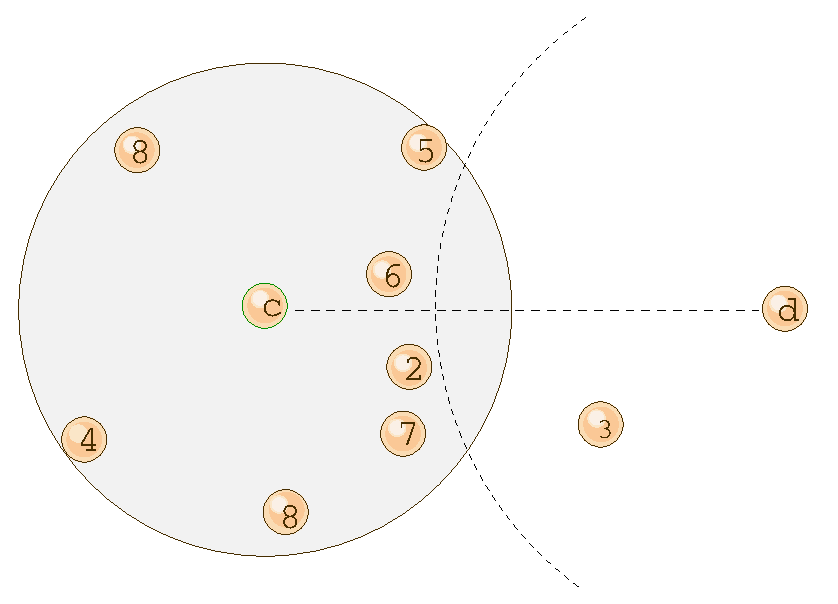
\includegraphics[width=2.6in]{progress}
  \caption{Illustration of several next nodes chosen by \(c\) using the progress-based forwarding strategies.}
  \label{fig:progress}
\end{figure}


\subsection{PAB3D}
\emph{PAB3D} is a randomized algorithm that tries to solve the local minimum problem described in previous section, by choosing the next node randomly from a subset of the current node's neighbors that makes progress to the destination. Already since 1984, some authors have tried to put the concepts of randomization algorithms in order to avoid the emergence of loops \cite{nelson:random, bose:compass, fevens:abface} using the concept of the random walk. Tipically, randomization performs as follow: let \(cw(u)\) be the neighbor node in \(N(c)\), over the line \(cd\), that minimizes one of the progress values defined in previous progress-based algorithms (distance, angle, etc.) and let \(ccw(u)\) be the neighbor node in \(N(c)\), under the line \(cd\), that minimizes the same one; then, randomized algorithms moves the packet to one of \{\(cw(u)\), \(cww(u)\)\} with equal probability or a probability weighted according to the progress values. Routing algorithms that use randomization are usually considered to fail when the number of hops in the path computed so far exceeds a threshold value, here called \(TTLR\) (\emph{Time To Live Random}).\\
Extension of randomized algorithm in 3D is not trivial, because it is not obvious to choose the best way to determine candidate neighbors. The reason is that in a three-dimensional graph there is no concept of above and below a line passing from source to destination. Therefore, in \cite{abdallah:random} authors propose an extension for the randomized-based algorithm from 2D to 3D, that uses the concept of 3D planes. This new algorithm is called \emph{AB3D} (\emph{Above/Below 3D}) and, instead of a line, it uses a plane to divide the 3D space in two choosing regions. In this document we generalize the concept of randomized-based algorithm defining a parametric algorithm, named \emph{PAB3D} (\emph{Parametrized AB3D}), that has four attributes:
\begin{itemize}
\item \(m\): are possible candidate neighbors to choose from \(N(c)\).
\item \(R\): is the name of progress-based strategy used to choose the \(m\) candidates, and it is one of \(R\) (Random), \(CM\) (Compass), \(GR\) (Greedy) or \(MF\) (most Forward), as in \emph{AB3D}.
\item \(S\): is used to represent the probability weighting when randomly choosing, and it is one of \(U\) (Uniform), \(D\) (Distance) , \(A\) (Angle), \(PD\) (Projection Distance). Probability weightings are defined as in \emph{AB3D}.
\item \(ab\) (above-below): is a boolean flag indicating whether to define the candidates over and below the Plane \(PL_1\) (or even over and below the plane \(PL_2\), if \(m = 5\)), or select candidates without considering the planes.
\end{itemize}
The main difference from \emph{AB3D} is the adding of parameter \(ab\), that selects if we have to use the plane or not.
The steps of the algorithm are the following. The current node \(c\) selects a node \(n_1\) from its neighbors, chosen according to the method defined in \(R\) (\(CM\), \(GR\) or \(MF\)). With \(ab = YES\), if \(m\) is \(3\), we define the plane \(PL_1\) identified by the three nodes \(s\), \(d\) and \(n_1\). If \(m\) is \(5\), define also the plane \(PL_2\) that is perpendicular to \(PL_1\) and passes through \(c\) and \(d\), such that the intersection line between the two planes is the line \(cd\). Fig. \ref{fig:ab3d} shows an example of network graph and its subdivision with the two planes.
Then, if the parameter \(m\) was \(3\), \emph{PAB3D} select another two nodes, in addition to \(n_1\). One neighbor \(n_2\) is chosen from the above of the plane \(PL_1\) according to \(R\) and one neighbor \(n_3\) is chosen from the below of the plane \(PL_1\) according to \(R\). If \(m\) was \(5\), in addition to \(n_1\), the algorithm choose from \(N(c)\) four neighbors \(n_2\), \(n_3\), \(n_4\), \(n_5\) each one in one side of the four regions that result from the intersection between \(PL_1\) and \(PL_2\). Once these candidates are determined, node \(c\) selects one of these nodes randomly, according to the probability weighting determined by \(S\), and forwards the packet to the chosen node.
Instead, with \(ab = NO\), the \(m\) candidates are chosen without a plane subdivision.

\begin{figure}[!t]
\centering
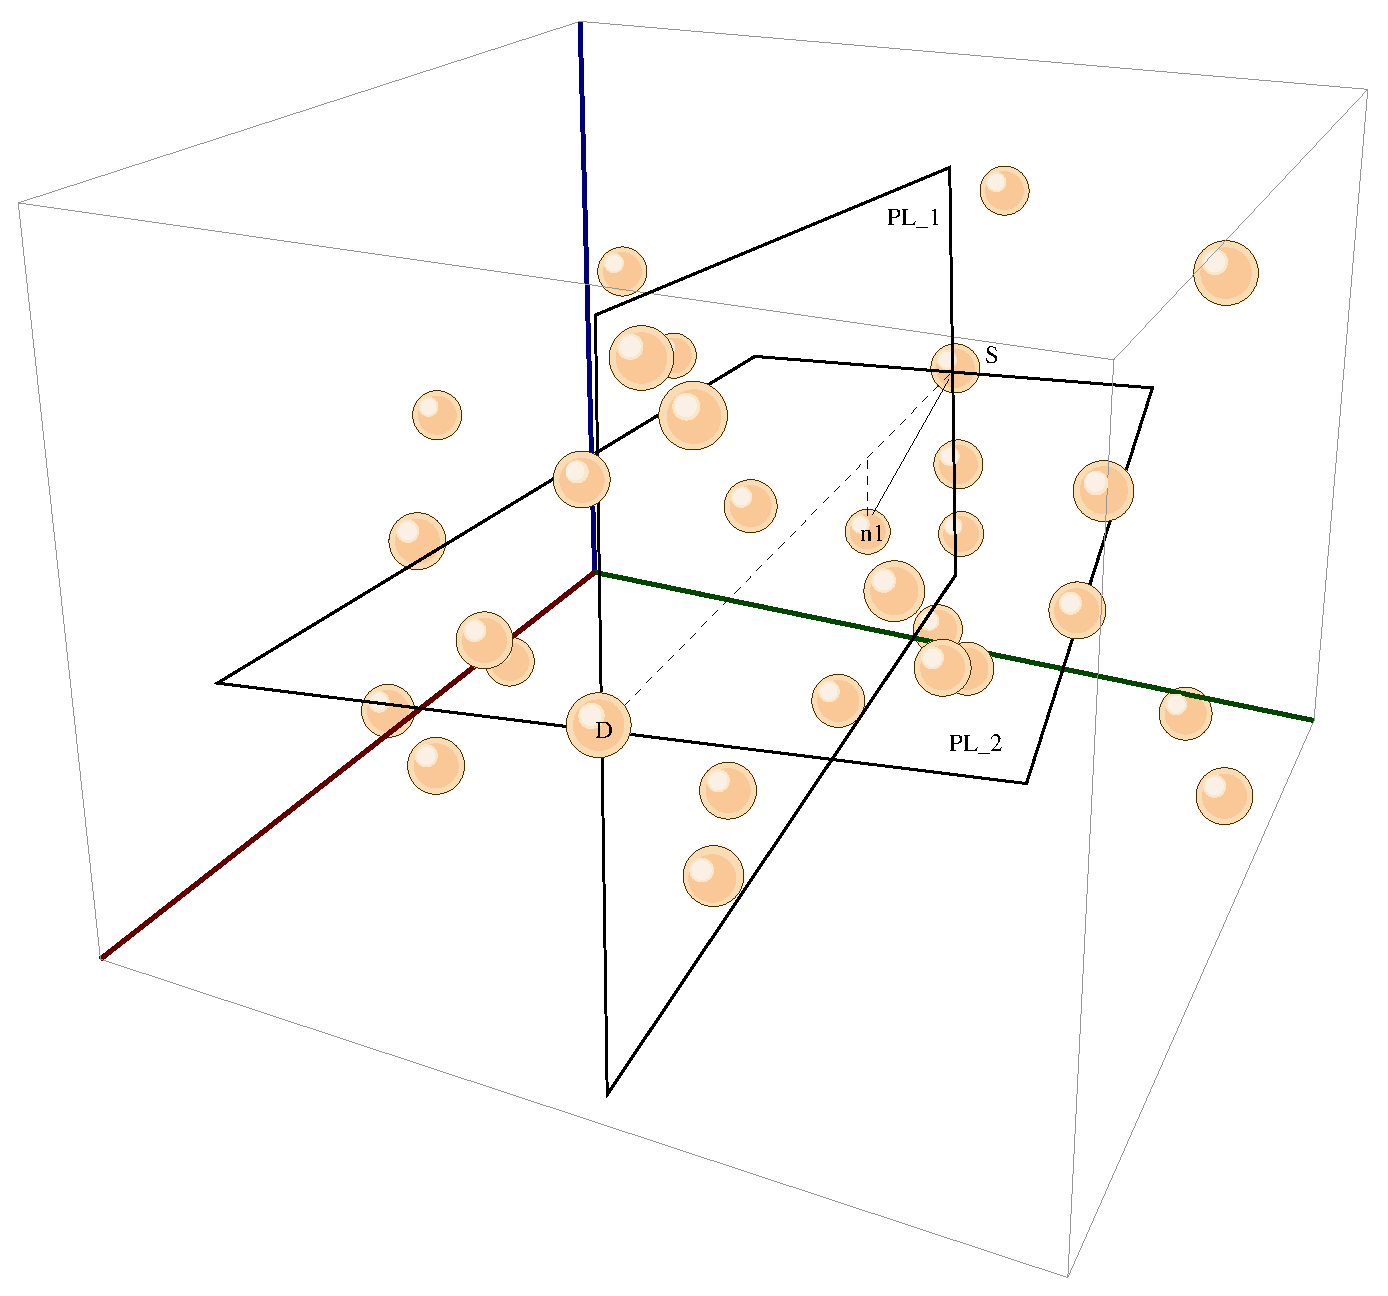
\includegraphics[width=3.0in]{images/ab3d}
\caption{In AB3D, plane \(PL_1\) passes through \(s\), \(d\) and \(n_1\), plane \(PL_2\) is orthogonal to \(PL_1\). Both planes contain the line \(sd\).}
  \label{fig:ab3d}
\end{figure}

\subsection{Greedy-Random-Greedy}
\emph{Greedy-Random-Greedy} (\emph{GRG}) algorithm belongs to \emph{progress-based/randomized-based} class, and uses \emph{Greedy} as the primary stage and a randomized algorithm, such as \emph{PAB3D}, as a recovery strategy. The general procedure of this algorithm is the following: the algorithm starts with the greedy phase until it finds a local minimum \(c\). At this point, \emph{GRG} stores the distance \(dist(c, d)\), and switches to the random phase, as recovery strategy, where the node \(c\) randomly selects one \(u\) of its neighboring nodes, using the steps defined in \emph{PAB3D}. If \(dist(u, d) < dist(c, d)\), then the algorithm resumes the greedy forwarding, otherwise continues with \emph{PAB3D}.

\subsection{Projective Face}
The first extension of face-based strategy in 3D space provides using two orthogonal planes intersected to the line connecting source and destination. In \cite{kao:3d} authors propose \emph{Projective Face}, in which the nodes of the networks are firstly projected onto one plane that contains the line \(sd\), with third point chosen randomly. Then, the \emph{Face} algorithm is performed on this projected graph. If the routing fails, the nodes are then projected onto a second plane, that is orthogonal to the first one and also contains the line \(sd\). Then, the \emph{Face} algorithm is again performed. Fig. \ref{fig:projectiveFace} shows an example of planes configuration in \emph{Projective Face}. Note that, in this case (and in all the following algorithms), since the delivery rate is not guaranteed, the algorithm needs a local threshold value, \(TTLF\) (\emph{Time To Live Face}), in order to terminate the algorithm in case it not reached the destination. This is necessary because the algorithm can get stuck in a loop. More precisely, in this version of algorithm, \(TTLF\) counter is started twice, once for the first plane and one for the orthogonal plane, obtaining a global threshold value, \(TTL \leq 2*TTLF\).

\begin{figure}[!t]
\centering
\includegraphics[width=2.6in]{images/projectiveFace}
\caption{Computing of a plane with \emph{Projective face} algorithm}
  \label{fig:projectiveFace}
\end{figure}

\subsection{CFace(3)}
\emph{CoordinateFace(3)} (\emph{CFace(3)}), proposed in \cite{abdallah:random}, uses another set of projection planes, that is composed by the planes \(xy\), \(xz\) and \(yz\) for the projection of the nodes. \emph{CFace(3)} works as follow. All nodes are projected on the first \(xy\) plane (\(node.z = 0\)) and then the face routing is started on the projected graph. If the packet does not arrive at the destination (\(TTLF\) has expired), the original coordinates of all nodes are projected on the \(xz\) plane (\(node.y = 0\)) and face routing is again performed. If again the packet does not arrive to the destination, the original coordinates of all nodes are projected on the \(yz\) plane (\(node.x = 0\)) and face routing is again performed. If the packet does not arrive even with this last plane, the algorithm fails. Fig. \ref{fig:cface} shows all the three projections on the coordinate planes. Note that, in this algorithm, \(TTL\) is at most \(3*TTLF\). As we will see, the delivery rate is typically greater than that of the \emph{Projective face}, but with also a greater path dilation.

\begin{figure}[!t]
\centering
\subfloat[\label{subfig:cface1}]{\includegraphics[width=1.3in]{images/cface1}}%
\subfloat[\label{subfig:cface2}]{\includegraphics[width=1.3in]{images/cface2}}%
\qquad
\subfloat[\label{subfig:cface3}]{\includegraphics[width=1.3in]{images/cface3}}%
\subfloat[\label{subfig:cface4}]{\includegraphics[width=1.3in]{images/cface4}}%
\caption{Projection of graph nodes (a) on the three planes \(xy\) (b), \(xz\) (c) and \(yz\) (d) in \emph{CFace(3)} algorithm.}
\label{fig:cface}
\end{figure}

\subsection{Adaptive Least-Square Projective Face}
Authors of \cite{kao:nearly} proposes three heuristics to modify and improve \emph{Projective Face} algorithm. The new obtained algorithm is called \emph{Adaptive Least-Squares Projective Face}, (\emph{ALSP Face}). The three heuristics are:
\begin{itemize}
\item Least-Squares Projection (LSP) Plane;
\item Adaptive Behavior Scale (ABS);
\item Multi-Projection-Plane Strategy.
\end{itemize}
 In the \emph{Projective Face} algorithm, a third point is chosen randomly, together with the source and the destination points, to compute the first projection plane. Instead, \emph{ALSP Face} chooses the third point adopting a mathematical optimization technique (first heuristic) for finding the best fitting plane to the set of neighbor nodes: using the current node, its neighbors up to two hops away, and the destination node, the initial projection plane is determined by using \emph{least-squares error minimization} of the distance of the nodes to the plane, hence minimizing the sum 
   \[  \sum^{m}_{i=1}(r_i)^2  \]
where \(r_i\) is the Euclidean distance from a point \(i\) to its perpendicularly projected point in the least-squares projection plane (\emph{LSP} plane), as seen in Fig. \ref{fig:lsp}. To maintain the local characteristic of the routing algorithm, authors propose that only the source, destination and the neighboring nodes within the 2-hops scope of the current node be selected as the set of points for computing the least projection plane \footnote{for simplicity of implementation, in this work the 1-hop scope of current node was used for \emph{LSP} plane computing} Then, nodes are projected on this plane and \emph{Face} routing is performed. This \emph{LSP} plane aims to have a less distorted projected graph so that the number of crossing edges can potentially be reduced. The second heuristic defines a parameter called \emph{Adaptive Behavior Scale} (\(ABS\)) that is used to determine when recalculate the \emph{LSP} plane, in order to ensure that the plan is always appropriate for the current node. The third heuristic uses a set of \(N_s\) projection planes arranged in a fixed order about an axis. The algorithm switches between these planes, following the order, to disrupt any looping that may occur during routing.
In \cite{kao:nearly} it is said that performing the face routing on the additional projection plane, significantly increases the delivery rate. Therefore, the third heuristic tries to increase the number of projection planes. But this is true only up to a certain point; even if it is true that the delivery rate is slightly increased, it is also true that the path followed by the packet becomes enormously long, because, for each projection plane, the threshold value (here, \(TTLF\)) is reset to its pre-set value. Such a high traffic for only one packet might not be acceptable in the real world. In this work we consider the third heuristic using only two additional planes, chosen as in \emph{Projective Face}.


\subsection{Greedy-Face-Greedy}
\emph{Greedy-Face-Greedy} algorithm (\emph{GFG}), also defined as \emph{Greedy Perimeter Stateless Routing} algorithm (\emph{GPSR}) for 2D networks, uses a combination of greedy method with face method.
With \emph{GFG}, a flag is stored in each data packet. This flag can be set into greedy-mode and face-mode (or perimeter-mode), indicating whether the packet is forwarded with \emph{Greedy} or \emph{Face} algorithm. The algorithm starts from \(s\) with \emph{Greedy}, setting the packet into greedy-mode and forwarding it. A node that receives a greedy-mode packet searches among its neighbors the node that is closest to the destination. If this neighbor exists, the current node forwards the packet to its, otherwise it marks the packet into perimeter-mode.
\emph{GFG} algorithm forwards the perimeter-mode packets performing the same planar graph as the \emph{Face2} algorithm. Moreover, when a packet enters in perimeter-mode at node \(x\), \emph{GFG} set the line \(xd\) as a reference line to the crossing with the faces and records in the packet the location of \(x\) as the node when greedy forwarding mode failed. This information is used at next hops to determine whether and when the packet can be returned to greedy-mode: upon receiving a perimeter-mode packet, the current node \(c\) first compares the location of \(x\) as stored in the packet with the forwarding node's location. \emph{GFG} returns in greedy-mode if the distance from the forwarding node to \(d\) is less than the distance from \(x\) to \(d\). In this case, the packet is set into greedy-mode and the algorithm continues greedy progress towards the destination. Fig. \ref{fig:gfg} shows an example, where the packet starts from \(s\) and travels \(x2\) and \(x3\) in greedy-mode, stopping at \(x3\), that is the local minimum. Then, from \(x3\), the face-mode is started, and forwards the packet on progressively closer faces of the planar graph, each of which is crossed by the line \(cd\). So, the packet reaches \(x4\), \(x5\) and \(x6\) in face-mode. \(x6\) is the closest node to \(d\) than \(x3\), so the packet can be returned to greedy-mode and reach \(d\).

\begin{figure}[!t]
\centering
\includegraphics[width=3.0in]{images/gfg}
\caption{Performing of \emph{GFG} algorithm. Solid arrows represent greedy-mode forwarding, dashes arrows represent face-mode forwarding.}
  \label{fig:gfg}
\end{figure}

\subsection{PAB3D-CFace(1)-PAB3D}
This algorithm, initially conceived in \cite{abdallah:random} as \emph{AB3D-CFace(1)-AB3D}, starts with \emph{PAB3D} algorithm. Once the local threshold \(TTLR\) is passed and the algorithm reaches a local minimum, it switches to \emph{CFace(1)}. \emph{CFace(1)} traverses one projective plane, which is chosen randomly from the \(xy\), \(yz\), or \(xz\) planes, starting from the node in which the algorithm is switched. At this point, \(TTLF\) is initialized to 0 and \emph{CFace(1)} restarts. If the destination is not reached during this phase and \(TTLF\) is passed (a looping occurs), the algorithm goes back to \emph{PAB3D} and \(TTLR\) restarts at 0.

\subsection{PAB3D-CFace(3)}
This algorithm starts as \emph{PAB3D-CFace(1)-PAB3D}, but instead of going back to \emph{PAB3D} if the phase in a projective plane fails, \emph{PAB3D-CFace(3)} tries the other two projective planes, defined as in \emph{CFace(3)}. This algorithm starts with the \emph{PAB3D} stage and if the destination is not reached and the \(TTLR\) is passed, the algorithm switches to \emph{CFace(3)} using the first \(xy\) plane. Again, if a loop occurred (\(TTLF\) is reached), it switches to \(yz\) plane, and finally the same process is done for \(xz\) plane.

\subsection{LAR 3D}
In the extension of \emph{LAR} algorithm in 3D space, with three-dimensional coordinates of source and destination positions, the source node computes the expected zone for \(d\), which is a sphere around \(d\) of radius equal to \(v_max * (t_1 - t_0)\) where \(t_1\) is the current time, \(t_0\) is the time stamp of the position information that c has about d, and \(v_max\) is the maximum speed of the node in the network. This zone is used to define the 3D flooding area, which is the minimum size rectangular box with \(ball(s,r)\) in one corner and the expected zone in the opposite corner. In our case, since we analyze static scenarios (\(v_max = 0\)), the expected zone is \(ball(d,r)\).

\subsection{PAB3D-LAR}
\emph{PAB3D-LAR} was proposed in \cite{abdallah:high} and hybridize \emph{PAB3D} with \emph{LAR}. This algorithm tries to reduce the high path dilation of the \emph{LAR} algorithm. All the combinations in \emph{PAB3D-LAR} use the same partitions as in the \emph{PAB3D} algorithm. The difference is that, while \emph{PAB3D} selects only one of the \(m\) candidates chosen from the neighborhood, \emph{PAB3D-LAR} sends the packet to all those selected candidates which are within the rectangular box defined as in \emph{LAR}.


\section{Performance Evaluation}
In this section we provide a performance comparison of the above considered routing protocols. A 3D simulation environment is structured for the experiment and a common set of configurations is provided.

\subsection{Simulation Environment}
Our simulation scenario consists of \textit{n} nodes placed in random positions in a 3D cubic space. The cube has 500 m of side length. Every scenario instance represents a connected networks, which means that each node can reach each other one. The node transmission range is set to 100 m. To simplify the simulation, we assume that the nodes are not moving, obtaining a static ad-hoc network. The motivation of this choice is twofold: (a) the need to consider initial essential parameters for the comparison (i.e. the minimum path) that would change if the nodes move, and (b) the assumption that, with the considered routing procotols, the route of each packet is traveled in a very little time, during which the nodes of the networks are essentially still. The first comparison aims to get a comprehensive look at the behavior of the forwarding algorithms under dinamyc number of nodes, ranging in \{50, 100, 150, 200\}. Second comparison analyzes the effect of varying the threshold values \emph{TTLR} and \emph{TTLF} of respectively randomized-based and face-based forwarding algorithms. The third comparison applies all the forwarding algorithms onto classes of graphs in which the length of the shortest path from source to destination ranges in 1-3 hops, 4-6 hops, 7-9 hops and 10+ hops (the notation \emph{a-b} indicates that the shortest path length in a-b class graph can assume values from \emph{a} to \emph{b} including).

\subsection{Results}
We discuss here the outcome of the experimentation and analyze the protocols' performances on different settings.
\subsubsection{Comparison with dynamic number of nodes}
First comparison performs considered routing protocols in a set of network istances consisting of 50, 100, 150, 200 nodes. The results are shown in Fig. \ref{fig:all_delivery} and \ref{fig:all_path}. From the results in Fig. \ref{fig:all_delivery}, we see immediately that deterministic progress-based forwarding algorithms have the lowest delivery rate, less than 60\% in the case of 150 nodes. This means that in this scenario (150 nodes) there is more chance of finding local minima. Instead, in the case of 200 nodes, we can see an increment of the delivery rate. This suggests a reduction of local minima with a growth of nodes' number starting from 150, in a cube of 500 meters of side length. The \emph{PAB3D} and \emph{G-PAB3D-G} algorithms obtain better results in delivery rate, with a peak in the case of 50 nodes (90\%), as seen in Fig. \ref{fig:all_50_delivery}. Face-based routing algorithms (\emph{Projective Face}, \emph{CFace(3)}, and \emph{ALSP Face}) have generally better results than the previous ones, in terms of delivery rate. This overcoming depends on the fact that these algorithts have more possibility to find the destination node, since \emph{TTLF} resetting. \emph{CFace(3)} can be defined as \emph{Projective Face}, only choosing two plans that are \emph{xy} plane and \emph{xz} plane, and with the addition of the \emph{xz} plane. So, since the algorithm has three chances to find the destination instead of two as in \emph{Projective Face}, the delivery rate is a little higher. The hybrid algorithm, \emph{GFG}, reaches better results compared to \emph{ALSP Face}, regarding delivery rate. This is caused probably by the greedy method phase that, at first, carries the packet towards the destination and then, if a local minimum is found, the face method phase starts, but with less search space. \emph{LAR} and \emph{PAB3D-LAR} are partial flooding-based algorithms. \emph{LAR} has relevant traffic and does not show a very high delivery rate. Not even \emph{PAB3D-LAR} presents a good delivery value, but has almost half of path dilation than \emph{LAR}. From what we can see in Figs. \ref{fig:all_150_delivery}, \ref{fig:all_200_delivery}, the transition from 150 nodes networks to 200 nodes ones increases the delivery rate, due to the increment of the node density and the restricion area includes many more nodes.


\begin{figure*}[!t]
\centering
\subfloat[]{\includegraphics[width=0.8\textwidth]{all_50_delivery}%
\label{fig:all_50_delivery}}

% where an .eps filename suffix will be assumed under latex, 
% and a .pdf suffix will be assumed for pdflatex; or what has been declared
% via \DeclareGraphicsExtensions.
\subfloat[]{\includegraphics[width=0.8\textwidth]{all_100_delivery}%
\label{fig:all_100_delivery}}


\subfloat[]{\includegraphics[width=0.8\textwidth]{all_150_delivery}%
\label{fig:all_150_delivery}}


\subfloat[]{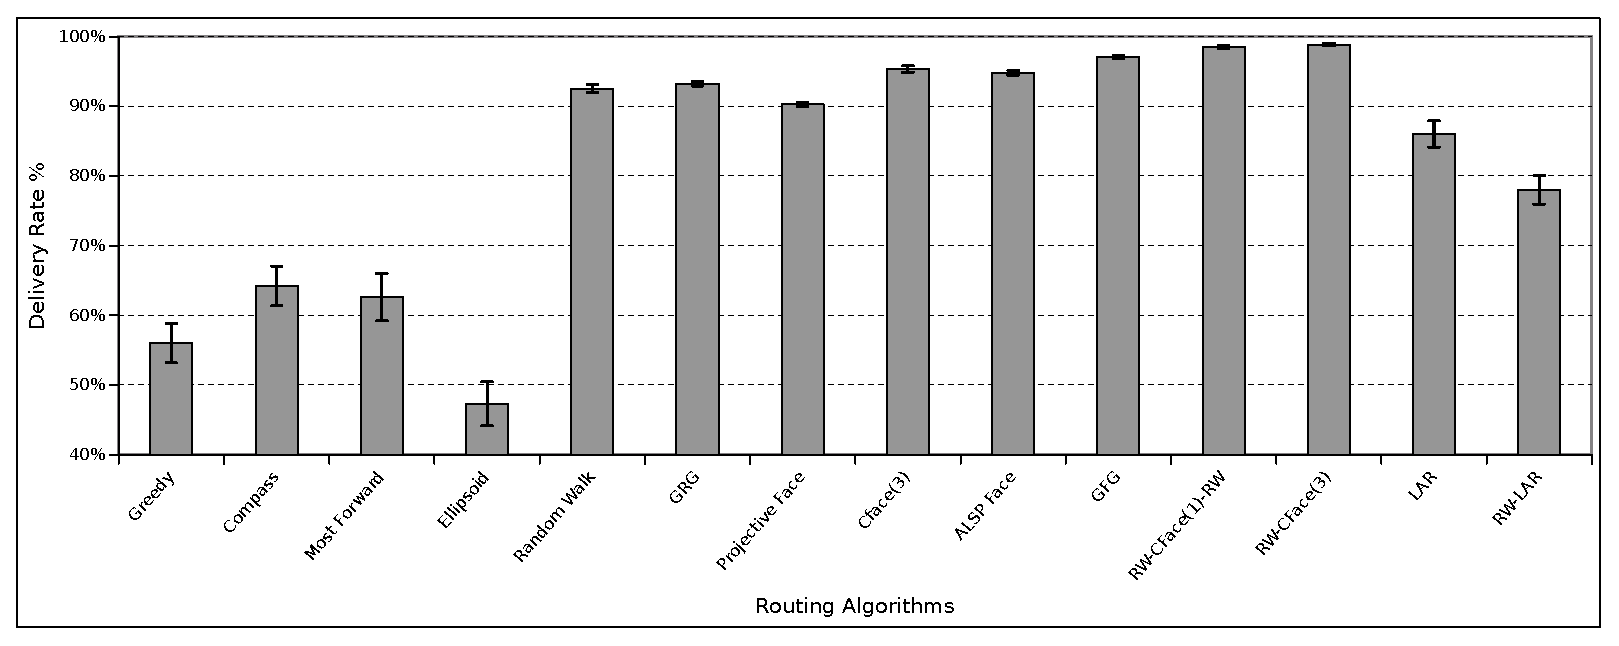
\includegraphics[width=0.8\textwidth]{all_200_delivery}%
\label{fig:all_200_delivery}}

\caption{Results of delivery rate}
\label{fig:all_delivery}
\end{figure*}

\begin{figure*}[!t]
\centering
\subfloat[]{\includegraphics[width=0.8\textwidth]{all_50_path}%
\label{fig:all_50_path}}

% where an .eps filename suffix will be assumed under latex, 
% and a .pdf suffix will be assumed for pdflatex; or what has been declared
% via \DeclareGraphicsExtensions.
\subfloat[]{\includegraphics[width=0.8\textwidth]{all_100_path}%
\label{fig:all_100_path}}


\subfloat[]{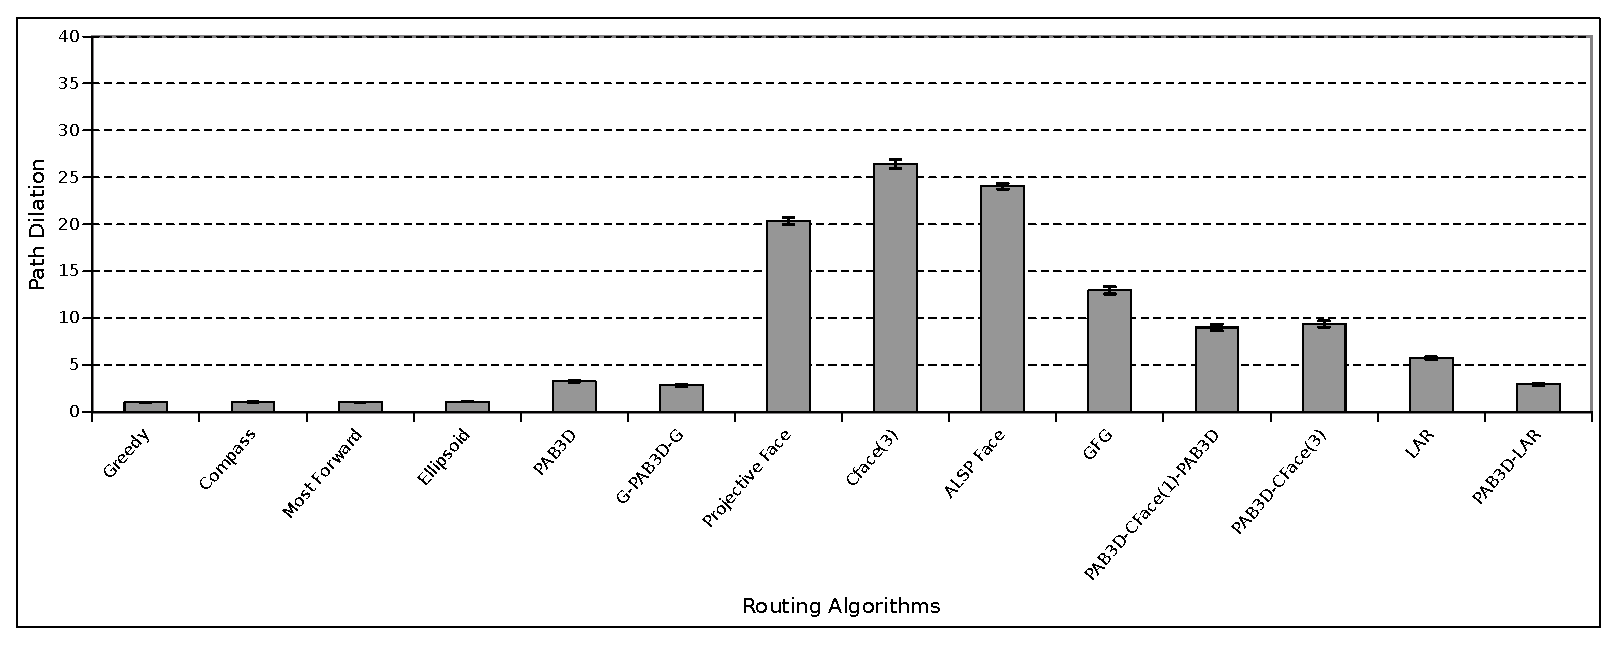
\includegraphics[width=0.8\textwidth]{all_150_path}%
\label{fig:all_150_path}}


\subfloat[]{\includegraphics[width=0.8\textwidth]{all_200_path}%
\label{fig:all_200_path}}

\caption{Results of path dilation}
\label{fig:all_path}
\end{figure*}

\subsubsection{Comparison with dynamic threshold values}
This performance test has the purpose of assessing the effect of the threshold values respectively for randomized-based and face-based algorithms, that is to see how effective is to increase the \emph{TTLR} and \emph{TTLF} values to increase delivery and path performance. In this test \emph{TTLR} and \emph{TTLF} are dynamic, while the number of nodes \emph{n} is not. Therefore, to get a fair treatment of the various instances and to allow each algorithm reach all their thresholds values (i.e., \emph{CFace(3)} fails after three times \emph{TTLF}), the \emph{TTL} value is calculated equal to \emph{2 * TTLR} for randomized case and to \emph{3 * TTLF} for face case.\\


\begin{figure*}[!t]
\centering
\subfloat[]{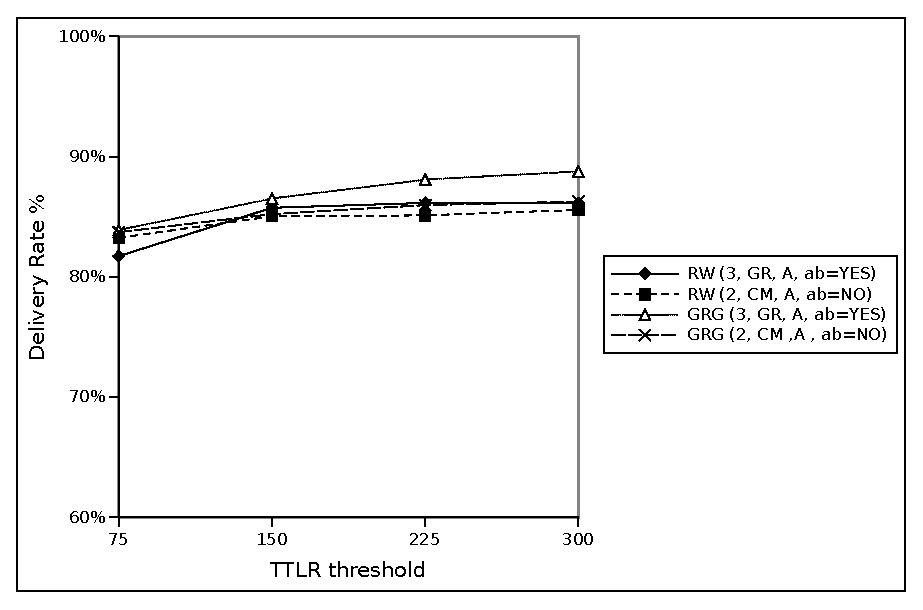
\includegraphics[width=0.8\textwidth]{test_5-13_change_TTLR_delivery}%
\label{fig:all_50_delivery}}

% where an .eps filename suffix will be assumed under latex, 
% and a .pdf suffix will be assumed for pdflatex; or what has been declared
% via \DeclareGraphicsExtensions.
\subfloat[]{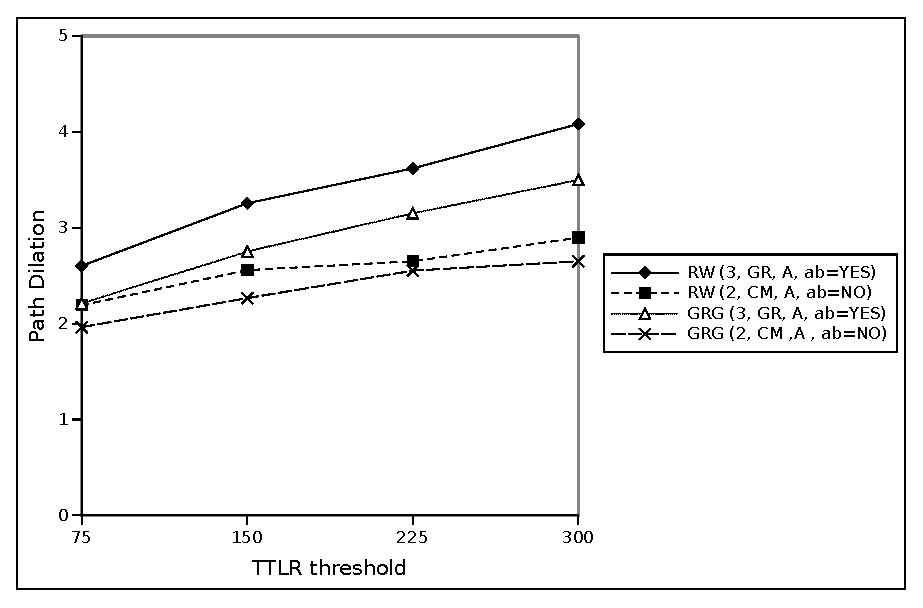
\includegraphics[width=0.8\textwidth]{test_5-13_change_TTLR_path}%
\label{fig:all_100_delivery}}
\end{figure*}

\begin{figure*}
\subfloat[]{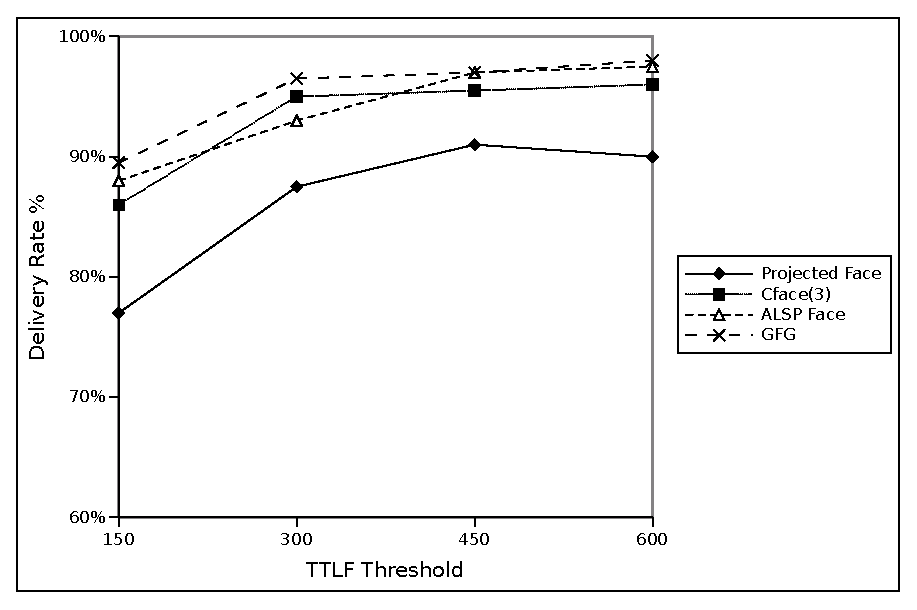
\includegraphics[width=0.8\textwidth]{test_7-8-9-10_change_TTLF_delivery}%
\label{fig:all_150_delivery}}


\subfloat[]{\includegraphics[width=0.8\textwidth]{test_7-8-9-10_change_TTLF_path}%
\label{fig:all_200_delivery}}

\caption{Results of path dilation}
\label{fig:all_delivery}
\end{figure*}


\subsubsection{Comparison with dynamic min path length}
This section shows the results relating to the application of all the routing algorithms considered in classes of graphs in which the length of the shortest path source-destination is respectively 1-3, 4-6, 7-9, and >10 hops. These results can be seen in Fig. \ref{fig:all_min_delivery}. Note that for the first class (1-3 hops, in Subfig. \ref{fig:all_min1-3_delivery}), all the algorithms have a high delivery rate and a small path dilation. This happens because there is very little chance that in a so few hops distance there are holes (local minima).
When it starts to move to longer paths, deterministic progress-based strategies are the first to degenerate, because, as the destination is more distant, there is a greater probability to find holes. As seen in Subfig. \ref{fig:all_min10_delivery}, progress-based algorithms reach about 10\% of delivery rate.
\emph{PAB3D} and \emph{GRG} perform well up to 4-6 length of minimum path, but from this point the delivery rate decreases. This is because the increasing number of links to choose from source to destination reduces the probability of choosing the righ path. However, the path length of the delivered packet remain short (see Subfig. \ref{fig:all_min4-6_delivery}, PAB3D and GRG histogram). The performance of face-based and hybridized algorithms are also good for high lengths, due to the fact that they succeed in reaching the destination within the \(TTLF\) or \(TTL\), despite the increasing of the distance from source to destination. However, the length of path performed is too high, due to an increment in the number of crossing links during the travel. \cite{IEEEhowto:kopka}

\begin{figure*}[!t]
\centering
\subfloat[]{\includegraphics[width=0.8\textwidth]{all_min1-3_delivery}%
\label{fig:all_min1-3_delivery}}

% where an .eps filename suffix will be assumed under latex, 
% and a .pdf suffix will be assumed for pdflatex; or what has been declared
% via \DeclareGraphicsExtensions.
\subfloat[]{\includegraphics[width=0.8\textwidth]{all_min4-6_delivery}%
\label{fig:all_min4-6_delivery}}


\subfloat[]{\includegraphics[width=0.8\textwidth]{all_min7-9_delivery}%
\label{fig:all_min7-9_delivery}}


\subfloat[]{\includegraphics[width=0.8\textwidth]{all_min10_delivery}%
\label{fig:all_min10_delivery}}

\caption{Results of delivery rate}
\label{fig:all_min_delivery}
\end{figure*}

\begin{figure*}[!t]
\centering
\subfloat[]{\includegraphics[width=0.8\textwidth]{all_min1-3_path}%
\label{fig:all_50_delivery}}

% where an .eps filename suffix will be assumed under latex, 
% and a .pdf suffix will be assumed for pdflatex; or what has been declared
% via \DeclareGraphicsExtensions.
\subfloat[]{\includegraphics[width=0.8\textwidth]{all_min4-6_path}%
\label{fig:all_100_delivery}}


\subfloat[]{\includegraphics[width=0.8\textwidth]{all_min7-9_path}%
\label{fig:all_150_delivery}}


\subfloat[]{\includegraphics[width=0.8\textwidth]{all_min10_path}%
\label{fig:all_200_delivery}}

\caption{Results of delivery rate}
\label{fig:all_delivery}
\end{figure*}



% Note that the IEEE typically puts floats only at the top, even when this
% results in a large percentage of a column being occupied by floats.


% An example of a double column floating figure using two subfigures.
% (The subfig.sty package must be loaded for this to work.)
% The subfigure \label commands are set within each subfloat command,
% and the \label for the overall figure must come after \caption.
% \hfil is used as a separator to get equal spacing.
% Watch out that the combined width of all the subfigures on a 
% line do not exceed the text width or a line break will occur.
%
%\begin{figure*}[!t]
%\centering
%\subfloat[Case I]{\includegraphics[width=2.5in]{box}%
%\label{fig_first_case}}
%\hfil
%\subfloat[Case II]{\includegraphics[width=2.5in]{box}%
%\label{fig_second_case}}
%\caption{Simulation results for the network.}
%\label{fig_sim}
%\end{figure*}
%
% Note that often IEEE papers with subfigures do not employ subfigure
% captions (using the optional argument to \subfloat[]), but instead will
% reference/describe all of them (a), (b), etc., within the main caption.
% Be aware that for subfig.sty to generate the (a), (b), etc., subfigure
% labels, the optional argument to \subfloat must be present. If a
% subcaption is not desired, just leave its contents blank,
% e.g., \subfloat[].


% An example of a floating table. Note that, for IEEE style tables, the
% \caption command should come BEFORE the table and, given that table
% captions serve much like titles, are usually capitalized except for words
% such as a, an, and, as, at, but, by, for, in, nor, of, on, or, the, to
% and up, which are usually not capitalized unless they are the first or
% last word of the caption. Table text will default to \footnotesize as
% the IEEE normally uses this smaller font for tables.
% The \label must come after \caption as always.
%
%\begin{table}[!t]
%% increase table row spacing, adjust to taste
%\renewcommand{\arraystretch}{1.3}
% if using array.sty, it might be a good idea to tweak the value of
% \extrarowheight as needed to properly center the text within the cells
%\caption{An Example of a Table}
%\label{table_example}
%\centering
%% Some packages, such as MDW tools, offer better commands for making tables
%% than the plain LaTeX2e tabular which is used here.
%\begin{tabular}{|c||c|}
%\hline
%One & Two\\
%\hline
%Three & Four\\
%\hline
%\end{tabular}
%\end{table}


% Note that the IEEE does not put floats in the very first column
% - or typically anywhere on the first page for that matter. Also,
% in-text middle ("here") positioning is typically not used, but it
% is allowed and encouraged for Computer Society conferences (but
% not Computer Society journals). Most IEEE journals/conferences use
% top floats exclusively. 
% Note that, LaTeX2e, unlike IEEE journals/conferences, places
% footnotes above bottom floats. This can be corrected via the
% \fnbelowfloat command of the stfloats package.




\section{Conclusion}
This survey had depeened, in many ways, the problem of position-based routing applied on three-dimensional networks. Firstly, the reasons of using an approach based on the position is discussed, and then the problems and limitations of the algorithms that use these techniques. 
\par Deterministic memoryless progress-based strategies can perform well in very dense networks, but not in a sparse networks, due to the problem of local minima. Algorithms that use this strategies, for instance \emph{Greedy}, may be used in combination with other algorithms, as seen, in order to reduce effectively the number of nodes traveled.
\par The random component in a forwarding decision offers a better chance to reach the destination. In this work, we have recovered all the randomized-based algorithms and unified them into a single algorithm called \emph{PAB3D}, with different input parameters. With a better combination of possible parameters, \emph{PAB3D} reaches a delivery rate of \%80, with a path length of at most three times the minimum path length in the considered scenarios. Hybridizing it with \emph{Greedy}, getting \emph{GRG}, there is not a significantly reduction of path dilation.





% if have a single appendix:
%\appendix[Proof of the Zonklar Equations]
% or
%\appendix  % for no appendix heading
% do not use \section anymore after \appendix, only \section*
% is possibly needed

% use appendices with more than one appendix
% then use \section to start each appendix
% you must declare a \section before using any
% \subsection or using \label (\appendices by itself
% starts a section numbered zero.)
%


\appendices
\section{Appendix 1}
Appendix one text goes here.

% Can use something like this to put references on a page
% by themselves when using endfloat and the captionsoff option.
%\if CLASSOPTIONcaptionsoff
  \newpage
%\fi



% trigger a \newpage just before the given reference
% number - used to balance the columns on the last page
% adjust value as needed - may need to be readjusted if
% the document is modified later
%\IEEEtriggeratref{8}
% The "triggered" command can be changed if desired:
%\IEEEtriggercmd{\enlargethispage{-5in}}

% references section

% can use a bibliography generated by BibTeX as a .bbl file
% BibTeX documentation can be easily obtained at:
% http://mirror.ctan.org/biblio/bibtex/contrib/doc/
% The IEEEtran BibTeX style support page is at:
% http://www.michaelshell.org/tex/ieeetran/bibtex/
\bibliographystyle{IEEEtran}
% argument is your BibTeX string definitions and bibliography database(s)
\bibliography{bibliography}
%
% <OR> manually copy in the resultant .bbl file
% set second argument of \begin to the number of references
% (used to reserve space for the reference number labels box)
\begin{thebibliography}{1}

\bibitem{IEEEhowto:kopka}
H.~Kopka and P.~W. Daly, \emph{A Guide to \LaTeX}, 3rd~ed.\hskip 1em plus
  0.5em minus 0.4em\relax Harlow, England: Addison-Wesley, 1999.

\end{thebibliography}

% biography section
% 
% If you have an EPS/PDF photo (graphicx package needed) extra braces are
% needed around the contents of the optional argument to biography to prevent
% the LaTeX parser from getting confused when it sees the complicated
% \includegraphics command within an optional argument. (You could create
% your own custom macro containing the \includegraphics command to make things
% simpler here.)
%\begin{IEEEbiography}[{\includegraphics[width=1in,height=1.25in,clip,keepaspectratio]{mshell}}]{Michael Shell}
% or if you just want to reserve a space for a photo:

\begin{IEEEbiography}{Claudio Enrico Palazzi}
Biography text here.
\end{IEEEbiography}

% if you will not have a photo at all:
\begin{IEEEbiographynophoto}{Armir Bujari}
Biography text here.
\end{IEEEbiographynophoto}

% insert where needed to balance the two columns on the last page with
% biographies
%\newpage

\begin{IEEEbiographynophoto}{Daniele Ronzani}
Biography text here.
\end{IEEEbiographynophoto}

% You can push biographies down or up by placing
% a \vfill before or after them. The appropriate
% use of \vfill depends on what kind of text is
% on the last page and whether or not the columns
% are being equalized.

%\vfill

% Can be used to pull up biographies so that the bottom of the last one
% is flush with the other column.
%\enlargethispage{-5in}



% that's all folks
\end{document}


\grid
\grid
